\subsection{M.PD.3 - Percentuale di requisiti opzionali soddisfatti}

\begin{figure}[H]
    \centering
    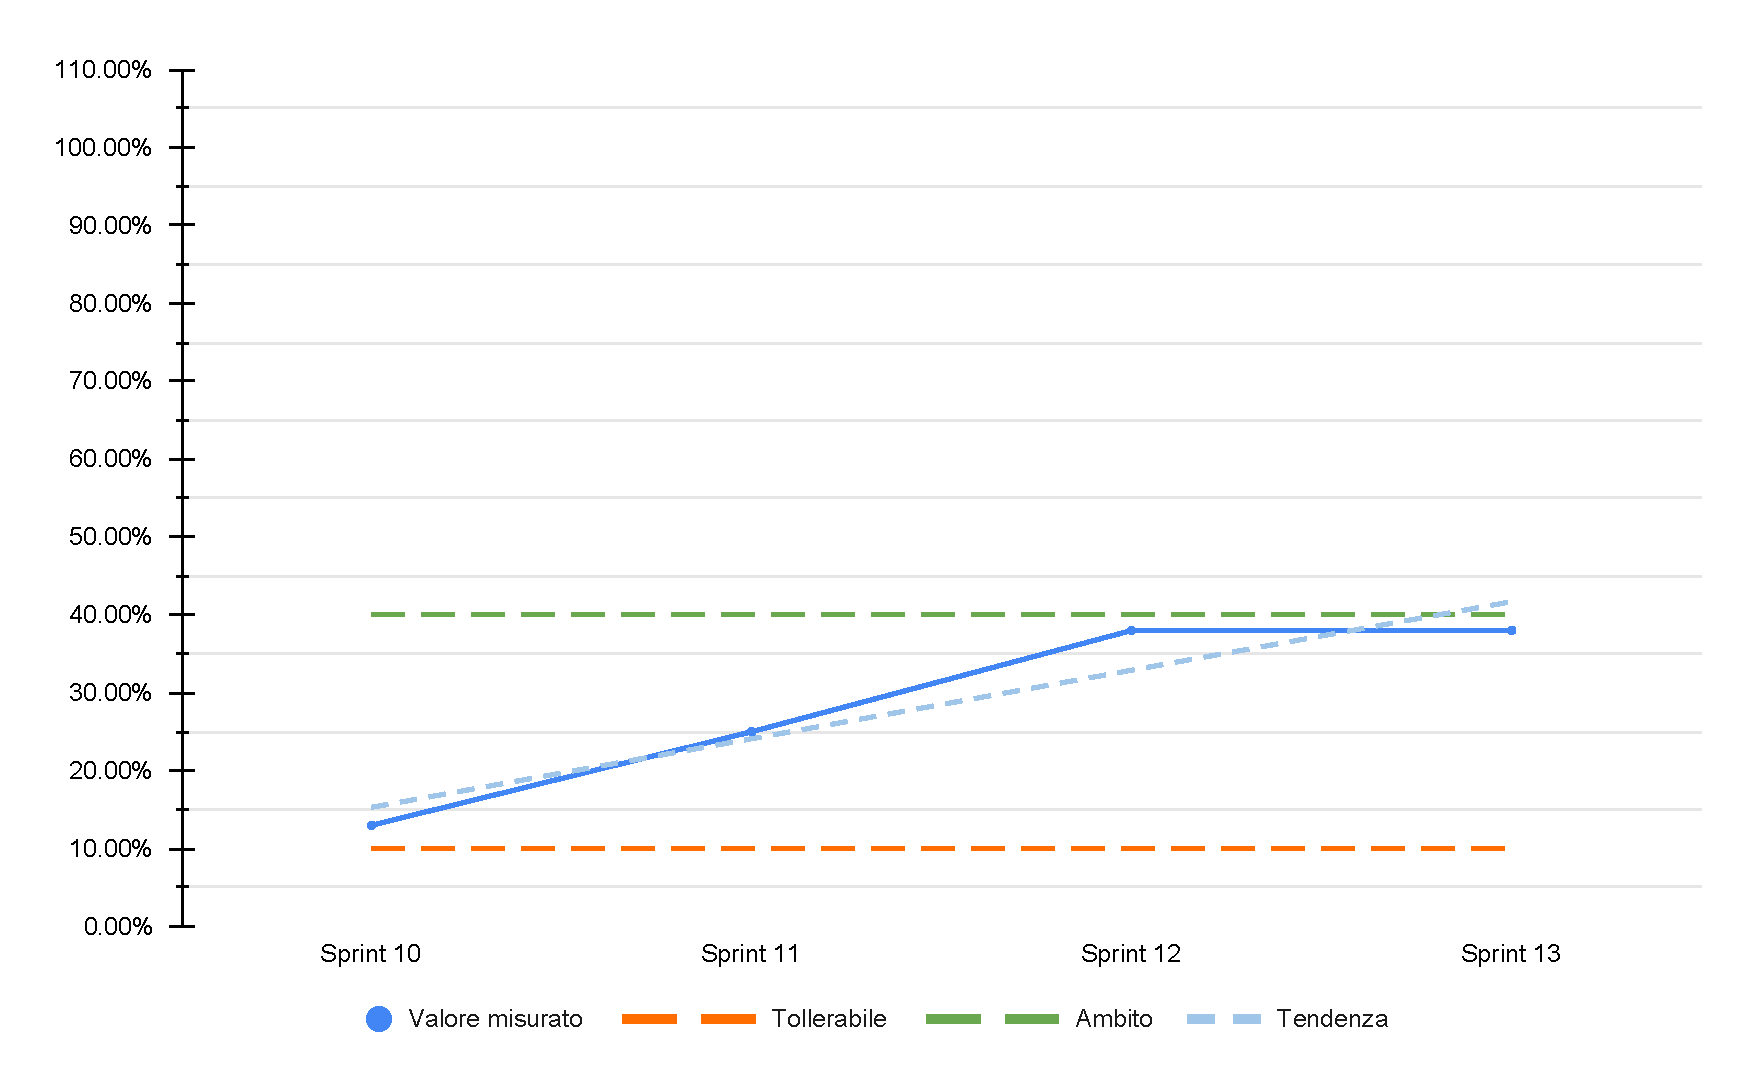
\includegraphics[width=\textwidth]{assets/requisiti_opzionali_soddisfatti.pdf}
    \caption{M.PD.3 - Percentuale di requisiti opzionali soddisfatti}
\end{figure}

\par Il team ha raggiunto una copertura dei requisiti opzionali inferiore al 50\%. Questo risultato è dovuto al fatto che alcuni di questi requisiti richiedevano un abbonamento a pagamento per accedere alle \glossario{API} dei modelli di intelligenza artificiale. Inoltre, il gruppo ha scelto di concentrarsi su funzionalità per le quali la \glossario{Proponente} ha manifestato interesse durante le riunioni, come il cambio lingua e il \glossario{debug} del \glossario{prompt}. Nonostante ciò, la copertura dei requisiti opzionali è rimasta entro un intervallo considerato accettabile.